\documentclass[a4paper,11pt,fleqn]{article}%fleqn pour aligner les equations à gauche
\usepackage{/home/rweye/Nextcloud/Documents/Overleaf/Styles/Exercice}

\newcommand{\chnum}{Chapitre 2}
\newcommand{\chtitle}{Composition des solutions aqueuses}
\newcommand{\dtype}{Exercices}

\begin{document}
\maketitle

\begin{multicols}{2}
\section{Bouillie bordelaise}
La bouillie bordelaise est utilisée pour combattre certains champignons qui attaquent les plantes. Des sites de jardinage donnent le mode d'emploi suivant pour en fabriquer :
\begin{itemize}
	\item mélanger \SI{80}{g} de chaux éteinte (hydroxyde de calcium \ce{Ca(OH)2(s)}
	\item mélanger \SI{150}{g} de sulfate de cuivre \ce{CuSO4(s)} dans \SI{5,0}{L} d'eau
	\item mélanger le tout dans un bidon de \SI{10}{L} au minimum
\end{itemize}
\begin{enumerate}
	\item S'agit-il d'une dilution ou d'une dissolution ?
	\item Quelle est la concentration finale en sulfate de cuivre ?
	\item Indiquer le protocole pour réaliser \SI{200}{mL} de bouillie.
	\item Quelles seront les précautions à prendre ? Justifier?
\end{enumerate}

\section{Le plein de vitamine C}
Un comprimé de vitamine C contient \SI{1000}{mg} d'acide ascorbique. Il se prend dans un verre d'eau de \SI{20}{cL}
\begin{enumerate}
	\item Une orange contient \SI{115}{mg} d'acide ascorbique. Combien faut-il d'oranges pour obtenir la même masse d'acide ascorbique que le comprimé ?
	\item Il faut environ trois oranges pour obtenir \SI{200}{mL} de jus. Quelle est la concentration en acide ascorbique du jus d'orange ?
	\item Quel volume de la solution obtenue avec le comprimé dans le verre contient la même masse d'acide ascorbique que ces trois oranges ?
	\item Quel volume d'eau faut-il ajouter au verre contenant le comprimé pour obtenir la même concentration en acide ascorbique que le jus d'orange ?
\end{enumerate}

\section{Précision d'un dilution}
On souhaite diluer 20 fois une solution commerciale de soude (hydroxyde de sodium) à \SI[separate-uncertainty = true]{10(1)}{\gram\per\liter}. On dispose d'une fiole jaugée de \SI[separate-uncertainty = true]{200.0(0.2)}{\milli\liter} et d'une pipette de \SI[separate-uncertainty = true]{10(0.04)}{\milli\liter}. L'incertitude sur la concentration de la solution fille $U(\gamma_{fille})$ est donnée par la relation suivante :
\begin{footnotesize} $$U(\gamma_{fille}) = \gamma_{fille} \sqrt{\left(\dfrac{U(\gamma_{mere})}{\gamma_{mere}}\right)^2 + \left(\dfrac{U(V_{mere})}{V_{mere}}\right)^2 + \left(\dfrac{U(V_{fille})}{V_{fille}}\right)^2}$$\end{footnotesize}
\begin{enumerate}
	\item Calculer l'incertitude sur la concentration de la solution diluée finale.
	\item Donner un encadrement de cette concentration.
\end{enumerate}

\section{Gel hydroalcoolique}
La formule de la solution hydroalcoolique développée par D. Pittet est mise à disposition de l'Organisation Mondiale de la Santé. Le mélange de liquides est le suivant (pour \SI{10}{L} finaux) : \SI{8.333}{L} d'éthanol à \SI{96}{\percent}, \SI{417}{mL} de solution de peroxyde d'hydrogène à \SI{3}{\percent}, \SI{174}{g} de glycérol à \SI{98}{\percent} et le reste est complété avec de l'eau distillée.
\begin{enumerate}
	\item Identifier le solvant dans la composition du gel hydroalcoolique.
	\item Quelle masse d'éthanol à \SI{96}{\percent} est utilisée pour \SI{10}{L} de solution ?
	\item Déterminer la masse volumique (en \unit{\gram\per\liter}) du gel.
\end{enumerate}

\textbf{Données :}\\
$\rho_{ethanol}$ = \SI{0,79}{\gram\per\centi\meter\cubed}\\
$\rho_{peroxyde}$ = $\rho_{eau}$\\
$\rho_{glycerol}$ = \SI{1.3}{\gram\per\milli\liter}

\section{Formation d'une cavité géologique}
Le Gouffre de Padirac, situé dans le Lot, est l’une des plus grandes curiosités géologiques de France. Cette cavité supposée cylindrique a un diamètre d’ouverture $d$ = \num{35} \unit{\meter} et une profondeur $h$ = \num{103} \unit{\meter}. Elle s’est progressivement formée par dissolution su carbonate de calcium \ce{CaCO3(s)} présent dans les roches calcaires dans l’eau de pluie s’infiltrant dans le sol. En moyenne, par an, on estime que le volume d’eau de pluie qui s’infiltre à travers une surface correspondant à celle de l’ouverture du gouffre est de l’ordre de \num{6e2} \unit{\meter \cubed} par an.\\
\textbf{Données :}
\begin{itemize}
	\item Volume d’un cylindre de hauteur $h$ et de rayon $R$ : $V = \pi \times R^2 \times h$
	\item Masse volumique du carbonate de calcium : $\rho_{\ce{CaCO3}}$ = \num{2,7e3} \unit{\gram \per \liter}
	\item Solubilité du carbonate de calcium dans la gamme de pH de l’eau de pluie de la région : $s$ = \num{0,30} \unit{\gram \per \liter}
\end{itemize}
\begin{enumerate}
	\item Calculer la masse de carbonate de calcium dissoute pour former le gouffre de Padirac
	\item En déduire le volume d’eau de pluie nécessaire pour dissoudre cette masse.
	\item En déduire une estimation du nombre d’années nécessaires à la formation d’une cavité de dimensions semblables à celles du gouffre de Padirac. Commenter.
\end{enumerate}
\vspace{1em}

\section{Prescription médicale}
Milla, trois ans est malade, elle a besoin de soins. Ses parents se rendent dans une pharmacie avec l’ordonnance du médecin.\\

\noindent \fbox{
\begin{minipage}{.98\linewidth}
\textbf{Document 1 : Ordonnance du médecin}\\
Zeclar : \num{15} \unit{\milli \gram} par \unit{\kilo \gram} de masse corporelle et par jour à répartir en deux prises pendant 5 jours.
\end{minipage}}


\noindent \fbox{
\begin{minipage}{\linewidth}
\textbf{Document 2 : Courbe de croissance de 0 à 3 ans}\\
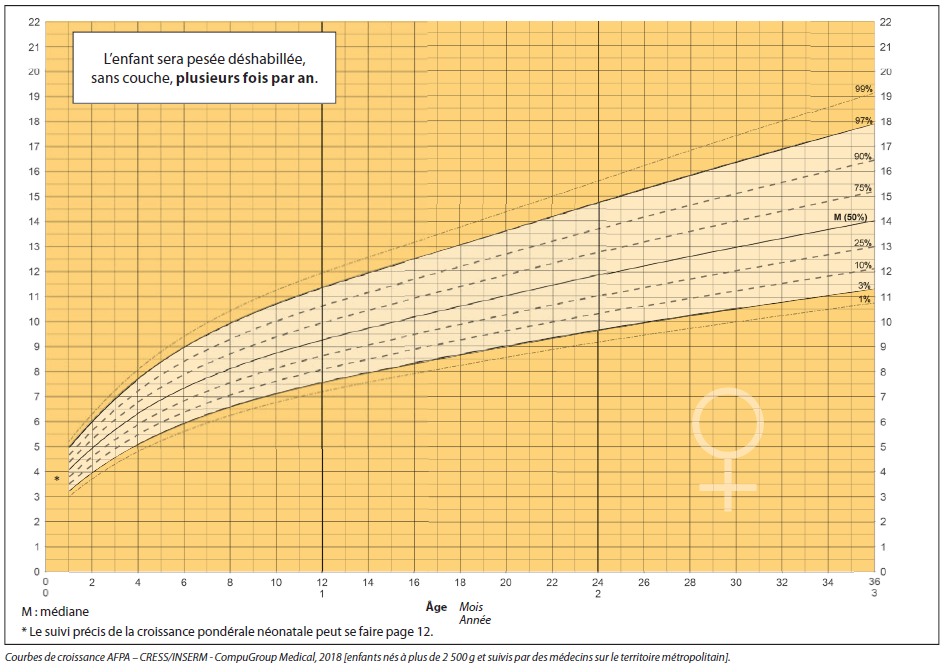
\includegraphics[width=\linewidth]{Ressources/2GT_C2_Ex_Fig2.png}
\end{minipage}}

\noindent\fbox{
\begin{minipage}{\linewidth}
\textbf{Document 3 : L’antibiotique prescrit}
\begin{center}
\begin{tabular}{|>{\centering}m{3.5cm}|>{\centering\arraybackslash}m{3.5cm}|}
\hline Antibiotique & Zeclar\\
\hline Forme galénique & Suspension buvable à reconstituer\\
\hline Concentration en masse du médicament reconstitué & \num{25} \unit{\gram \per \liter}\\
\hline Volume de la solution reconstituée flacon & \num{100} \unit{\milli \liter}\\
\hline Mode d’administration & Seringue graduée de 1 à 8 kg\\
\hline
\end{tabular}
\end{center}
\end{minipage}}

\textbf{Question :}
Déterminer combien de flacons la pharmacienne doit délivrer aux parents de Sarah, sachant que la courbe de croissance de Sarah se situe dans la moyenne.
\end{multicols}

\end{document}